%\documentclass[letterpaper, 12pt]{report}
\documentclass[letterpaper, 11pt]{article}

%\usepackage{float}
%\floatplacement{figure}{H}

%\author{Brian Bell}
%\date{2-10-2013}
%\title{Humans as Property in the Early West: \\ Contrasting the Origins and Operation of Russian Serfdom with the Peculiar Instituton of Slavery in the United States.}
%\affiliation{2102055378 \\ HST-104 (10162)}


%\usepackage[dvips]{graphicx}
%\usepackage[pdftex]{graphicx}
\usepackage{graphicx}
%\usepackage[dvipdfmx]{graphicx}
\DeclareGraphicsExtensions{.eps,.pdf,.jpg,.png}

%\usepackage[caption=false,labelfont=sf,textfont=sf,captionskip=5pt]{subfig}

%\DeclareGraphicsRule{.pnXg}{eps}{.bb}{}

\usepackage{achicago}
\usepackage{fullpage}
%\usepackage[top=1in, bottom=1in, left= 1 in, right=1in]{geometry}
%\usepackage[top=1.5in, bottom=1.5in, left=1.5in, right=1in]{geometry}
\usepackage{geometry}

%\usepackage{diagbox}

% *** MATH PACKAGES ***
%
%\usepackage{amsmath}
\usepackage[cmex10]{amsmath}
\usepackage{amsfonts}
\usepackage{mathtools}
% A popular package from the American Mathematical Society that provides
% many useful and powerful commands for dealing with mathematics. If using
% it, be sure to load this package with the cmex10 option to ensure that
% only type 1 fonts will utilized at all point sizes. Without this option,
% it is possible that some math symbols, particularly those within
% footnotes, will be rendered in bitmap form which will result in a
% document that can not be IEEE Xplore compliant!
%
% Also, note that the amsmath package sets \interdisplaylinepenalty to 10000
% thus preventing page breaks from occurring within multiline equations. Use:
%\interdisplaylinepenalty=2500
% after loading amsmath to restore such page breaks as IEEEtran.cls normally
% does. amsmath.sty is already installed on most LaTeX systems. The latest
% version and documentation can be obtained at:
% http://www.ctan.org/tex-archive/macros/latex/required/amslatex/math/





% *** SPECIALIZED LIST PACKAGES ***
%
 \usepackage[ruled, boxed]{algorithm2e}
 \usepackage{algorithmic}

%\usepackage{natbib}
%\usepackage[natbib=true, bibstyle=authoryear, citestyle=authoryear-comp]{biblatex}

% for distance between bib items
\usepackage{bibspacing}
\setlength{\bibitemsep}{1.0\baselineskip plus .05\baselineskip minus .05\baselineskip}

%\usepackage[super,sort&compress]{natbib}

\usepackage{layout}

\usepackage{setspace}


\usepackage[nopar]{lipsum} % for dummy text
\usepackage[american]{babel}
\usepackage[babel]{csquotes}
%\usepackage{natbib}
%\usepackage[notes,natbib,isbn=false,backend=biber]{biblatex-chicago}
%\addbibresource{bibfile.bib}

\usepackage{fancyhdr}

%\fancyhf{}
%\fancyhead[C]{\thepage}
%\pagestyle{fancy}

% redefine the plain pagestyle
%\fancypagestyle{plain}{%
%\fancyhf{} % clear all header and footer fields
%\fancyhead[C]{\thepage} % except the center
%}

%\usepackage{chicago}
%\usepackage{fancyhdr}
\pagestyle{fancy}
%\fancyhead[R]{Humans as Property in the Early West - \thepage}
\fancyhead[R]{\thepage}
\fancyfoot{}
\renewcommand{\headrulewidth}{0pt}
\renewcommand{\footrulewidth}{0pt}


%\newcommand{\HRule}{\rule{\linewidth}{0.25mm}}
\newcommand{\HRule}{\rule{\linewidth}{0mm}}

\doublespacing
%\setlength{\parindent}{0pt}

% 36pt == 0.5in


\setlength{\voffset}{0in}
\setlength{\hoffset}{0in}

\setlength{\marginparpush}{0in}
\setlength{\footskip}{0in}

\setlength{\marginparsep}{0in}
\setlength{\marginparwidth}{0in}

\setlength{\textheight}{578pt}
\setlength{\textwidth}{434pt}



%\setlength{\oddsidemargin}{0.5in}

\setlength{\topmargin}{0in}
\setlength{\headheight}{0in}
\setlength{\headsep}{0.5in}

\setlength{\footnotesep}{24pt}
%\setlength{\skip\footins}{0pt}

%\setlength{\parindent}{4em}

%\setlength\bibitemsep{1.5\itemsep}
%\setlength{\bibitemsep}{1.5in}


\begin{document}%\layout
\begin{titlepage}
\begin{center}

\HRule

\textbf{\Huge Machine Learning 101} \\
\bigskip\bigskip\bigskip\bigskip\bigskip\bigskip\bigskip\bigskip\bigskip\bigskip\bigskip
{Group 11: Bide Xu (260711367)}\\
{Mengjia Gu (260790140)}\\
{Robin Luo (260851506)}\\
\bigskip\bigskip\bigskip\bigskip\bigskip\bigskip\bigskip\bigskip\bigskip\bigskip\bigskip
{Course Number: COMP 551}\\
{Course Name: Applied Machine Learning}\\
{\today}

\end{center}
\end{titlepage} 

\clearpage
\setcounter{page}{2}
%\autocite{citekey} just use footnotes!

\singlespacing

\begin{abstract}
Online posts and forums have become increasingly popular in daily use and valuable in marketing support. Hence, prediction on comment popularity is explorable for more applications. This project was purposed to assess the performance of linear regression models for predicting comment popularity on Reddit. Given the pre-crawled dataset, we applied two approaches of linear regression models, closed-form solution and gradient descent, to prediction models with and without text features. Although we modified value of hyperparameters in gradient descent and tried to improve performance, the closed-form solution actually runs faster and presents more accurate and stable results.

In addition, an improved version of gradient descent algorithm is also implemented, by introducing a new parameter called ``distance rate'', which helps to let the learning rate value keep a reasonable distance from the epsilon value, so that the learning rate would not decay too quick. Therefore, this ``distance rate'' could help the algorithm run a reasonable enough time in order to improve the accuracy of the result (evaluated in MSE). This ``distance rate'' cooperates well with the Robbins Monroe logic, so could assist to achieve a well balance between run-time and accuracy.

Furthermore, new text feature based on 60 or 160 most high frequency words in the training data is implemented, with significant improvement for the prediction of popularity score. Also, other new implemented text feature such as ``average words per sentence'' indeed reduced MSE (mean square errors) of models and hence improved performance. Another new numeric feature is also implemented, which is the ``cubic of children field'' -- $children^3$. Both of these new designed features perform well in the improvement of the accuracy w.r.t both training data and validation data.

Moreover, we also implemented punctuation removing and stop words filtering features, though they did not bring obivious performance improvement according to our experiment.

\end{abstract}

\section*{Introduction}

Discussion board is frequently used in academic communication, product review and other public message exchange. This variety of information, which serves as a data source of the predicting technique, contributes to commercial development in recommendation system design\cite{rohlin2016popularity}. Reddit is a classic and popular discussion platform, connecting communities with various topics. This project is proposed to construct and compare linear regression models in purpose of predicting comment popularity on Reddit. We are given some prepared data of selected comments, which still required preprocessing before import into experiments. Three features (children, controversiality, is\_root) and one output variable are directly from the original dataset. Other input variables, such as text features and word counts, were extracted or derived from text content of comments.

Given the pre-crawled dataset, we preprocessed data, extracted features, and built models for both closed-form solution and gradient descent. Not as the theoretical expectation, out experiment results illustrated that, compared to gradient descent method, closed-form solution is better in both runtime and accuracy. Compared models differently implemented with text features, we noticed that involving text content of a comment into models obviously improved the accuracy of prediction on popularity. By adding new input variables like ``average number of words per sentence'', we deduced the significance of comment content in prediction of popularity.

\section*{Dataset}

The original dataset consists of 12,000 data points in format of dictionary. Each dictionary contains five keys with different types of value. Data in each type of information forms one or more variables in linear regression models. We translated some of them in format better support linear regression models, as described below:

\begin{itemize}
    \item popularity\_score: numeric output variable, larger value means more popular comment
    \item children: non-negative integers indicate number of replies received
    \item controversiality: binary metric, 0 means not controversial and 1 means controversial comment
    \item is\_root: binary, True represents a direct comment instead of being a reply, and contrary for False
    \item text: text content of a comment, which is convert to lower case and split by space, to generate new features
\end{itemize}

Besides the popularity\_score representing how popular each comment is, other information are taken as input variables that may affect prediction results. Text features are drawn from a wordlist of most frequently used words in all given comments. This wordlist contains 160 words ranking by occurrences in text content of comments. We as well count total number of words of comment and average word per sentence in each text value in order to add them as new features improving prediction.

After preparing features, we divided dataset into three parts for different purposes: first 10000 for data training, next 1000 as a validation set, and last 1000 to test model. Considered the limitation of data source, out project may lose accuracy lacking data of more features like post topics and timeline. Failures in measuring popularity score could also lead to missing objectiveness and reliability of our data source. Moreover, user preference is always difficult to detect, especially that Reddit targets on public audience with various backgrounds.

\section*{Results}

All our experiment results are stored as .json file, which will be submitted with the source codes and other documents. The performance for different added features are summerized in Table \ref{tbl:table_fp}, and discussed as following:

\subsection*{Closed-Form Solution v.s. Gradient Descent}

Simply with non-text features directly extracted from dataset, closed-form solution without extra hyperparameter stands out for its stability and smaller mean square errors of both training and validation sets. Besides input variables, three hyperparameters affected results by gradient descent. Firstly, we determined how often should we change the learning rate: suppose the learning rate change every T iteration. Then in experiment, we set the value of $\epsilon$ to $10^{-6}$, the value of $\eta$ to 1. We found that MSE does not affected by the value of T, but running time is the lowest when T equals to $10^{2}$, therefore, we set the value of T to $10^{2}$. Secondly, we determined the value of $\epsilon$, MSE does not change much after $\epsilon$ is less than $10^{-5}$. However, the running time is increasing as the value of epsilon decreasing. Therefore, we set the value of $\epsilon$ to $10^{-5}$. Finally, we determined the value of $\eta$, while eta increasing, MSE is decreasing. The maximum eta is 1, therefore we set the value of $\eta$ to 1.

Lowering learning rate took longer time to reduce mean square errors, while decreasing run time ended experiment before reaching small mean square errors, as discussed in Figure \ref{fig:cf_vs_gd}. The new implemented hyperparameter ``distance rate'' was added to introduce some balance between speed and accuracy, although it could not outperform the ideal model with closed-form solution, it indeed provided a well balanced solution to solve the conflict between runtime and accuracy, bring better accuracy, almost $ 10^{-10} $ in MSE regarding the ideal weight vector [[-0.22627679][-1.08584747][0.37536403][0.82092517]] obtained by the closed form method, compared to the normal version of Gradient Descent method, as detailed in Figure \ref{fig:cf_vs_2gd}.

\subsection*{Word Count Features}

Implemented with the closed-form solution, models using text features from the high frequency words list took longer time to present lower MSE on both training and validation sets. Our experiment results show that the 60 words version could improve the MSE of validation data from 1.0203 to around 0.9693, while the improvement of 160 words version(s) are not as stable as the 60 words version(s), which have similar improvement in MSE for training set and validation set as the 60 words version(s), but do not perform well in the testing set.
 
\subsection*{New Features}

The ``average number of words per sentence'' feature obiviously reduced the MSE of linear regression models in predicting comment popularity, from 1.0203 to around 1.0127 for the validation data. This text feature is selected due to its performance is better than some other text features we have attempted, such as ``total number of words in the comment'', ``total number of sentence'' and ``average length per word''. Although the ``total number of words'' feature does bring some degree of stable optimization, but its improvement is less than 0.005 in MSE, and therefore is not selected in our final model.

Also, we implemented word filters to remove punctuations, this feature does reduce MSE in some degree, but the improvement is not significant enough. However, we find that it is interesting when combine this feature together with the high frequency word count feature as well as other text features, for it could help to increase the stability of the prediction accuracy improvement of other text features.

The new numeric feature of ``$children^3$'' is also helpful to optimize the accuracy, the improvement is from 1.0203 to 1.0024 in MSE for the validation data. All these two new added features also work well for the training data.

\subsection*{Performance for Combined features}

When the word frequency, the ``average number of words per sentence'' and the ``$children^3$'' features are integrated together, our experiment shows that their improvement can be combined well, which improve the MSE of the validation data from 1.0203 to around 0.9473 in total. This overall improvement is also verified by the testing data, whose MSE can be reduced from 1.2975 to 1.2631.

\section*{Discussion and Conclusion}

This project indicated better results of linear regression models with closed-form solution than which with gradient descent, which against the theoretical suggestion of better performance by gradient descent. One possible explanation is that small size of dataset, requiring only few operations, cannot reflect the advantage of gradient descent in dealing with huge data and complex operations.

More and better filtered text features improve the prediction accuracy. Other features derived from text data, like comment length and word counts per sentence, better predict the comment popularity as well. Newly added features are also related to text content of comments. Therefore, text content significantly affects the popularity of a comment. Meanwhile, more text features take models longer time to run experiments.

More features in reality should be considered as important variables affecting how popular a comment on Reddit is. The idea of predicting comment popularity facilitates in technical development in commercial area, especially through improving recommendation systems.

\section*{Contribution Statement}

All members brainstormed for data preparation, feature extraction, and model construction.
\begin{itemize}
    \item Bide Xu: main python coding
    \item Robin Luo: models improvement and graph plotting
    \item Mengjia Gu: results test and summarize write-up
\end{itemize}

All participated in whole progress and learnt through this project.


\nocite{*}

\bibliographystyle{achicago}



\begingroup

    %\setlength{\bibsep}{10pt}

    \setstretch{1}
    \bibliography{bibfile}


\endgroup
%\renewcommand{\baselinestretch}{2.1}
\renewcommand{\thepage}{}

%\bibliography{bibfile}

%\setlength{\bibitemsep}{1.5itemsep}
%\setlength{\bibnamesep}{1.5itemsep}
%\setlength{\bibinitsep}{1.5itemsep}



%\pagestyle{fancy}
%\fancyhead[R]{\thebibliography}
%\fancyfoot{}
%\renewcommand{\headrulewidth}{0pt}
%\renewcommand{\footrulewidth}{0pt}


%\begin{figure}
%  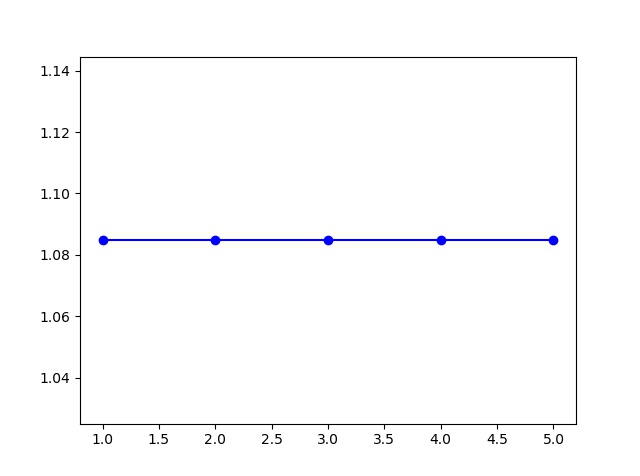
\includegraphics[width=\linewidth]{fig/pic1.jpg}
%  \caption{Relationship among }
%  \label{fig:relation1}
%\end{figure}



\begin{figure}[!ht]
  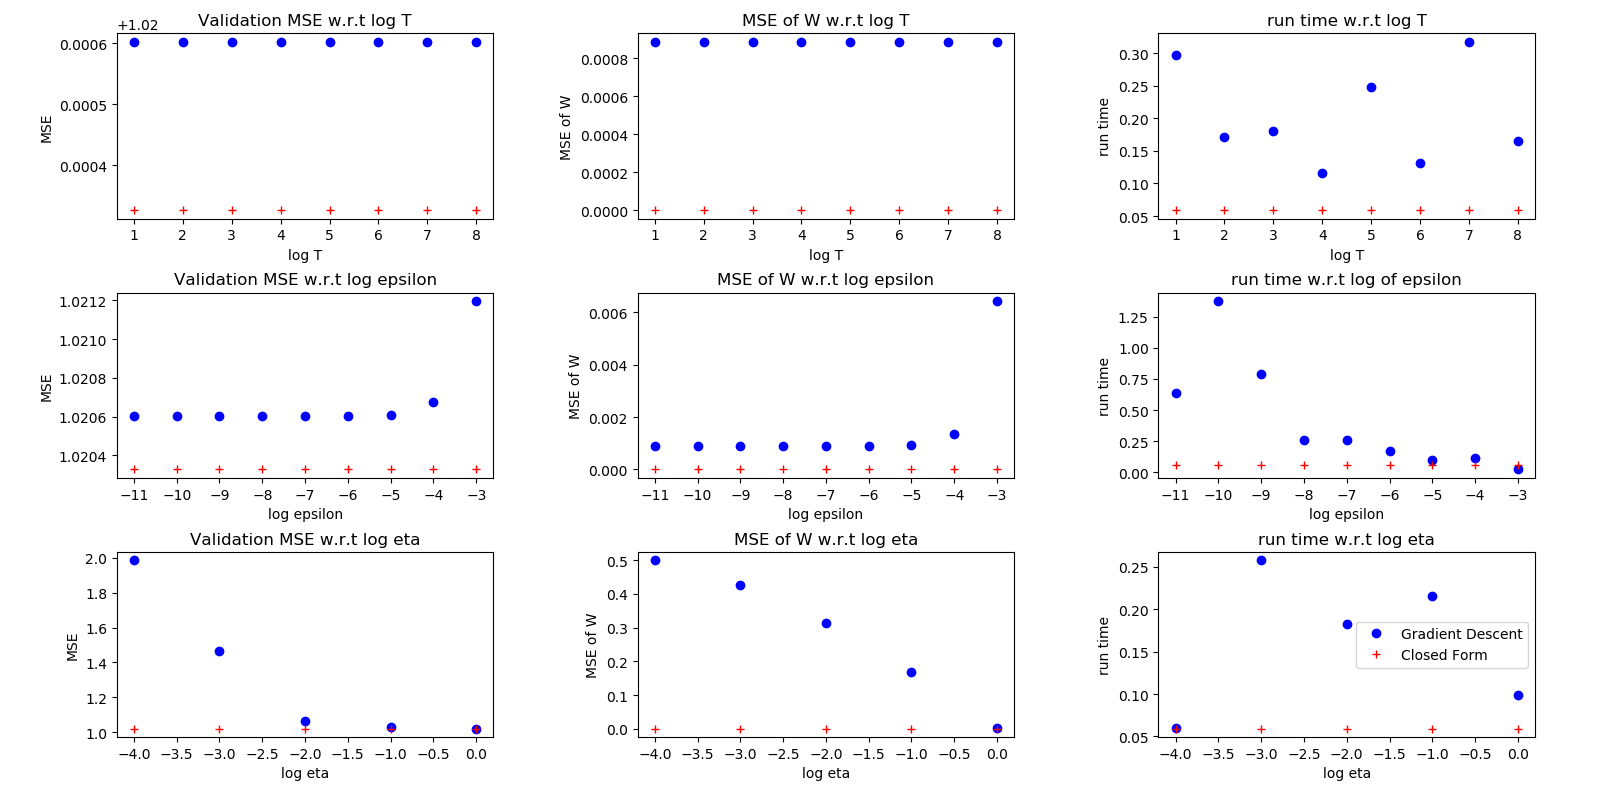
\includegraphics[width=\linewidth]{fig/figure_cf_vs_gd.png}
  \caption{run time, accuracy performance comparsion between closed Form Alg and Gradient Descent Alg, the stability of Gradient Descent Alg varies w.r.t different initial settings of its hyperparameters, such as period (T) of Robbins Monroe, $\epsilon$ and $\eta$. While the performance of the Closed Form Alg is stable.}
  \label{fig:cf_vs_gd}
\end{figure}


\begin{figure}[!ht]
  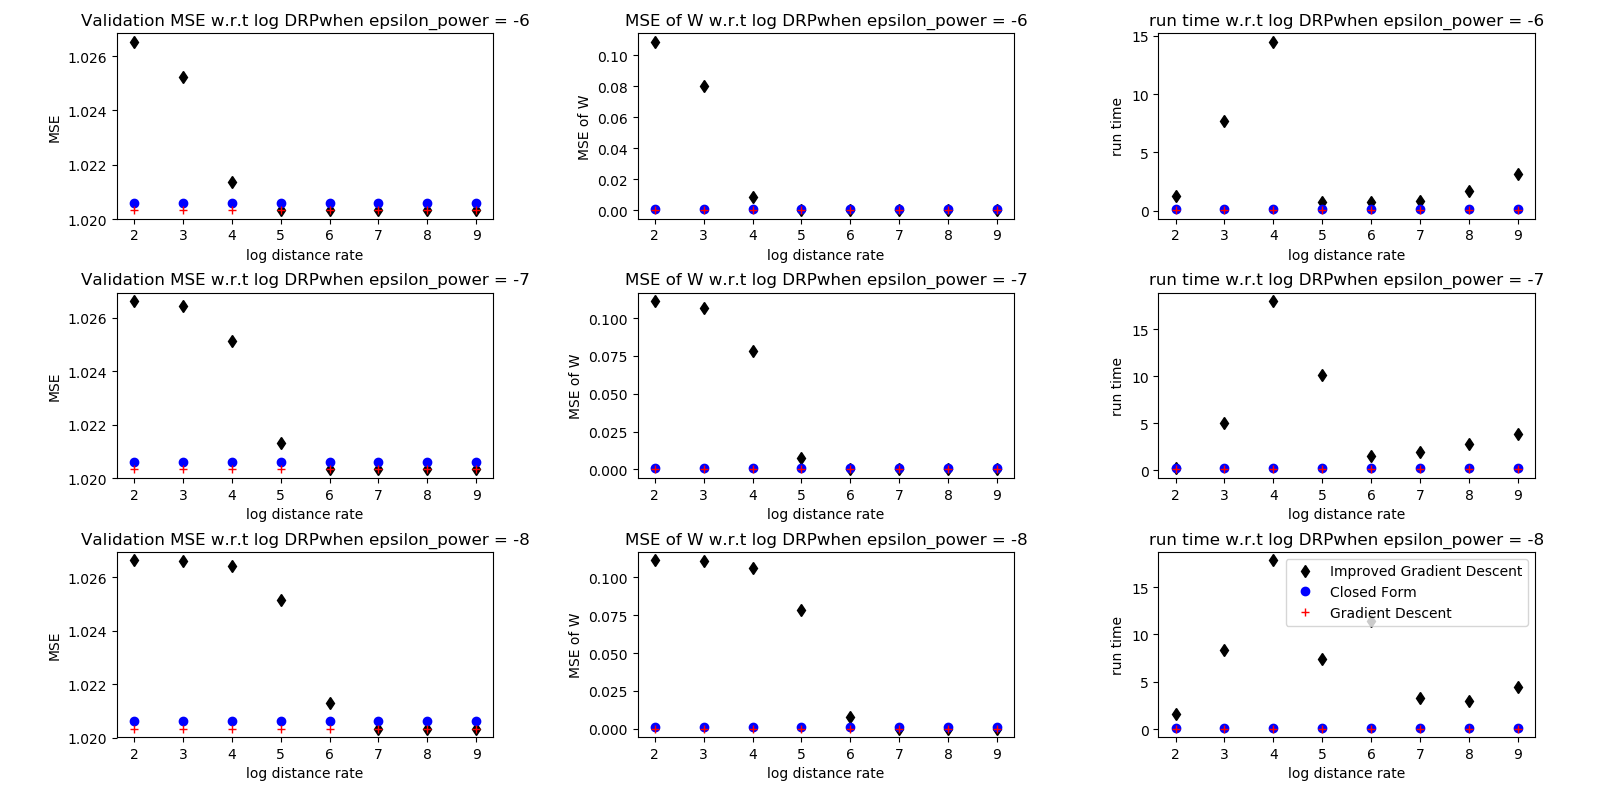
\includegraphics[width=\linewidth]{fig/figure_cf_vs_2_gd_revised.png}
  \caption{run time, accuracy performance comparsion between closed Form Alg, Gradient Descent Alg and Improved Gradient Descent Alg, with $\epsilon$ value around $10^{-6}$ to $10^{-8}$. Those figures shows than, when the distance rate is more than 4, in other words, roughly $10^{4}$ larger then the $\epsilon$ value, the accuracy for the Improved Gradient Descent Alg starts to outperform the normal Gradient Descent Alg and become very near to the ideal results obtained by the closed form Alg. So the improved Gradient Descent Alg could be more accurate than the original Gradient Descent Alg, with acceptable more runtime.}
  \label{fig:cf_vs_2gd}
\end{figure}

\begin{table}[]
\centering
\begin{tabular}{|l|l|l|l|l|l|}
\hline
\textbf{Feature(s) w.r.t Performance}                                                                                                                                     & \textbf{\begin{tabular}[c]{@{}l@{}}MSE of \\ Training \\ Data\end{tabular}} & \textbf{\begin{tabular}[c]{@{}l@{}}MSE of \\ Validation \\ Data\end{tabular}} & \textbf{\begin{tabular}[c]{@{}l@{}}MSE of \\ Testing \\ Data\end{tabular}} & \textbf{\begin{tabular}[c]{@{}l@{}}run time \\ (in S)\end{tabular}} & \textbf{\begin{tabular}[c]{@{}l@{}}pre-run time \\ (in S) \\ time for \\ computing \\ text/numeric \\ features\\ and generate \\ related matrix\end{tabular}} \\ \hline
\textbf{\begin{tabular}[c]{@{}l@{}}Basic Model \\ (3 numeric  features)\end{tabular}}                                                                                     & 1.084683                                                                    & 1.020326                                                                      & 1.297531                                                                   & 0.027982                                                            & 3.207755                                                                                                                                                      \\ \hline
\textbf{Model With:}                                                                                                                                                      &                                                                             &                                                                               &                                                                            &                                                                     &                                                                                                                                                               \\ \hline
\textbf{“60 high frequency  words”}                                                                                                                                       & 1.059316                                                                    & 0.969286                                                                      & 1.298629                                                                   & 0.026985                                                            & 88.564367                                                                                                                                                     \\ \hline
\textbf{\begin{tabular}[c]{@{}l@{}}“60 high frequency words”\\ + “remove punctuation”\end{tabular}}                                                                       & 1.061179                                                                    & 0.983503                                                                      & 1.285445                                                                   & 0.149432                                                            & 79.076935                                                                                                                                                     \\ \hline
\textbf{“160 high frequency words”}                                                                                                                                       & 1.047630                                                                    & 0.996385                                                                      & 1.318918                                                                   & 0.891486                                                            & 185.632877                                                                                                                                                    \\ \hline
\textbf{\begin{tabular}[c]{@{}l@{}}“160 high frequency  words” \\ + “remove punctuation”\end{tabular}}                                                                    & 1.046506                                                                    & 0.983375                                                                      & 1.318479                                                                   & 0.099944                                                            & 193.501532                                                                                                                                                    \\ \hline
\textbf{Model With:}                                                                                                                                                      &                                                                             &                                                                               &                                                                            &                                                                     &                                                                                                                                                               \\ \hline
\textbf{“average words per sentence”}                                                                                                                                     & 1.081087                                                                    & 1.012782                                                                      & 1.288209                                                                   & 0.015989                                                            & 3.331969                                                                                                                                                      \\ \hline
\textbf{\begin{tabular}[c]{@{}l@{}}“average words per sentence”\\ + “remove punctuation”\end{tabular}}                                                                    & 1.081173                                                                    & 1.013062                                                                      & 1.288329                                                                   & 0.000998                                                            & 3.996707                                                                                                                                                      \\ \hline
\textbf{Model with:}                                                                                                                                                      &                                                                             &                                                                               &                                                                            &                                                                     &                                                                                                                                                               \\ \hline
\textbf{“$Children^3$”}                                                                                                                                    & 1.041047                                                                    & 1.002414                                                                      & 1.267450                                                                   & 0.001998                                                            & 3.309102                                                                                                                                                      \\ \hline
\textbf{\begin{tabular}[c]{@{}l@{}}“$Children^3$” \\ + “average words per sentence”\end{tabular}}                                                          & 1.037979                                                                    & 0.995746                                                                      & 1.258209                                                                   & 0.002000                                                            & 4.707468                                                                                                                                                      \\ \hline
\textbf{\begin{tabular}[c]{@{}l@{}}“$Children^3$” \\ + “average words per sentence”\\  + “remove punctuation”\end{tabular}}                                & 1.038087                                                                    & 0.995989                                                                      & 1.258282                                                                   & 0.001997                                                            & 3.371063                                                                                                                                                      \\ \hline
\textbf{All text features:}                                                                                                                                               &                                                                             &                                                                               &                                                                            &                                                                     &                                                                                                                                                               \\ \hline
\textbf{\begin{tabular}[c]{@{}l@{}}“60 high frequency words” \\ + “average words per sentence”\end{tabular}}                                                              & 1.057966                                                                    & 0.966220                                                                      & 1.294168                                                                   & 0.219871                                                            & 67.993910                                                                                                                                                     \\ \hline
\textbf{\begin{tabular}[c]{@{}l@{}}“60 high frequency words” \\ + “average words per sentence” \\ + “remove punctuation”\end{tabular}}                                    & 1.059723                                                                    & 0.979785                                                                      & 1.280751                                                                   & 0.023983                                                            & 62.781974                                                                                                                                                     \\ \hline
\textbf{\begin{tabular}[c]{@{}l@{}}All Combined:\\ text \& numeric features\end{tabular}}                                                                                 &                                                                             &                                                                               &                                                                            &                                                                     &                                                                                                                                                               \\ \hline
\textbf{\begin{tabular}[c]{@{}l@{}}“$Children^3$” \\ + “60 high frequency words” \\ + “average words per sentence”\end{tabular}}                           & 1.015920                                                                    & 0.947381                                                                      & 1.263172                                                                   & 0.020987                                                            & 69.911887                                                                                                                                                     \\ \hline
\textbf{\begin{tabular}[c]{@{}l@{}}“$Children^3$” \\ + “60 high frequency words” \\ + “average words per sentence” \\ + “remove punctuation”\end{tabular}} & 1.017403                                                                    & 0.959957                                                                      & 1.253317                                                                   & 0.021993                                                            & 65.182590                                                                                                                                                     \\ \hline
\end{tabular}
\caption{Performance Evaluation For Varies Implemented Features and Their Combinations}
\label{tbl:table_fp}
\end{table}


\end{document} 